\section{Simple Titles}

As we learned in Chapter \ref{chapter:oop}, we can add a title with the axes method \code{set_title()}. Simply pass the string of your choice as the argument. For multi-line titles, recall \code{\\n} can be used in a string to start a new line. Common optional arguments include \code{color}, \code{fontsize}, \code{weight}, and \code{loc}. 

Colors will be addressed in Chapter \ref{chapter:colors}, but to start you can simply use the name of any not-too-exotic color as a string.

\code{fontsize} (or \code{size}) can be a number or chosen from \code{'small'}, \code{'medium'}, or \code{'large'}, and \code{'small'} and \code{'large'} may be intensified with a \code{'x-'} or \code{'xx-'} prefix. Similarly, \code{weight} (or \code{fontweight}) can be a number or chosen from options like \code{'bold'} or \code{'light'}.

\code{loc} determines the location of the title, either \code{'left'}, \code{'center'}, or \code{'right'}. In the default style, the default value will be \code{'center'}. You might prefer using \code{'left'} to match the Google Sheets default (thus matching the vast majority of plots I've seen in industry). %Consider using \code{'left'} to match the Google Sheets default. 
\code{pad} controls the space between the title and the top of the axes. 


\pyfile{title-pad.py}

\begin{center}
    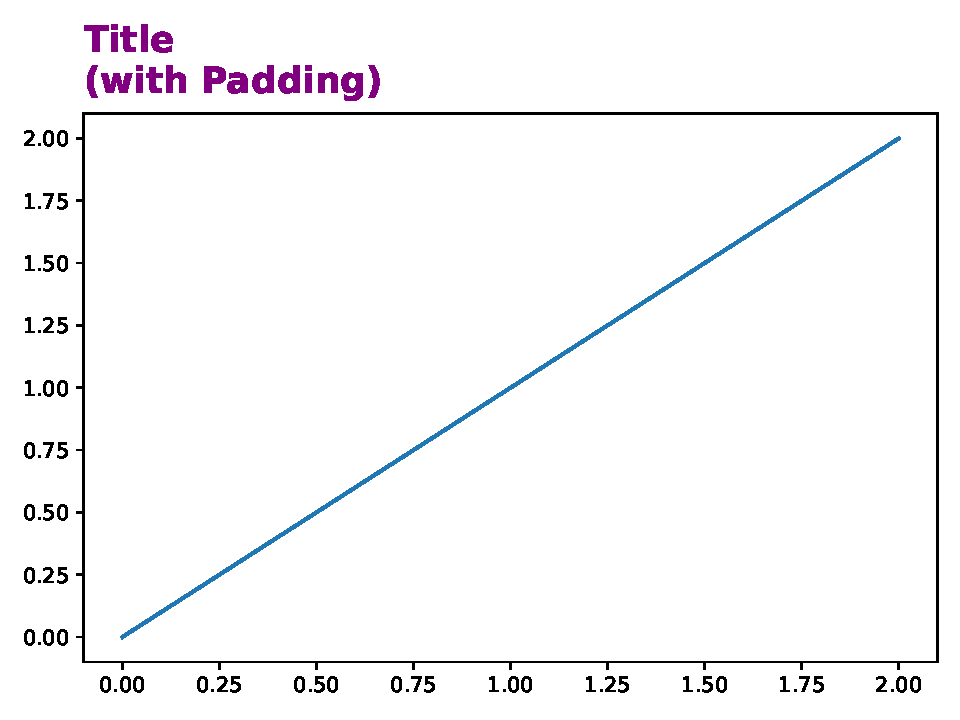
\includegraphics[width = .48\textwidth]{figures/proseplots/title-pad.pdf}
\end{center} \begin{center}
    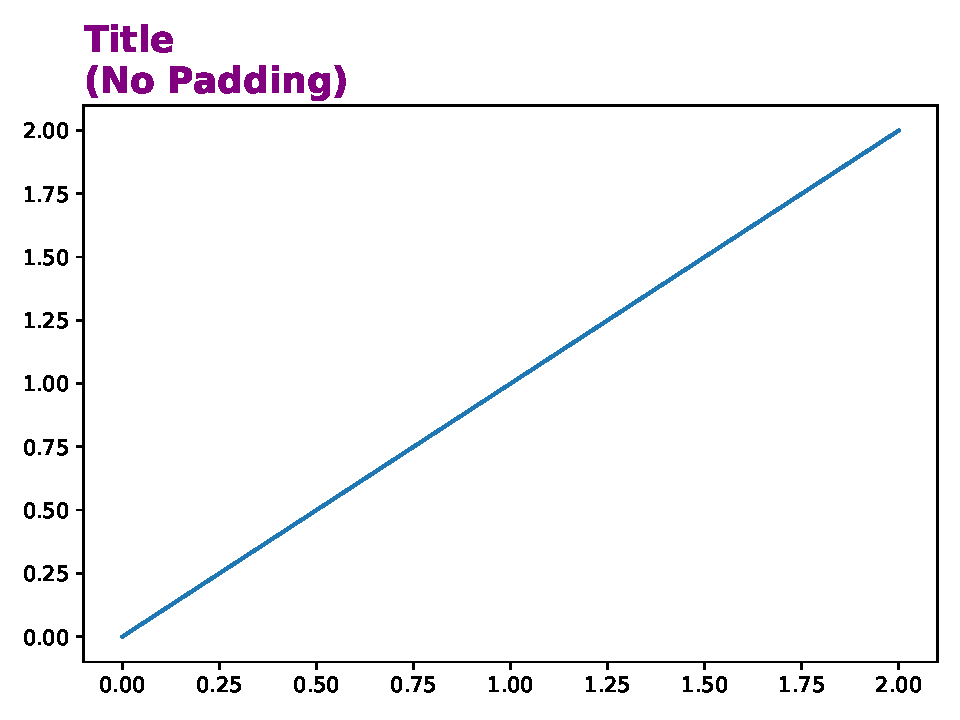
\includegraphics[width = .48\textwidth]{figures/proseplots/title-no-pad.pdf}
\end{center}

A plot can actually have one title for every \code{loc} value as well. 

\pyfile{title-loc.py}

\begin{center}
    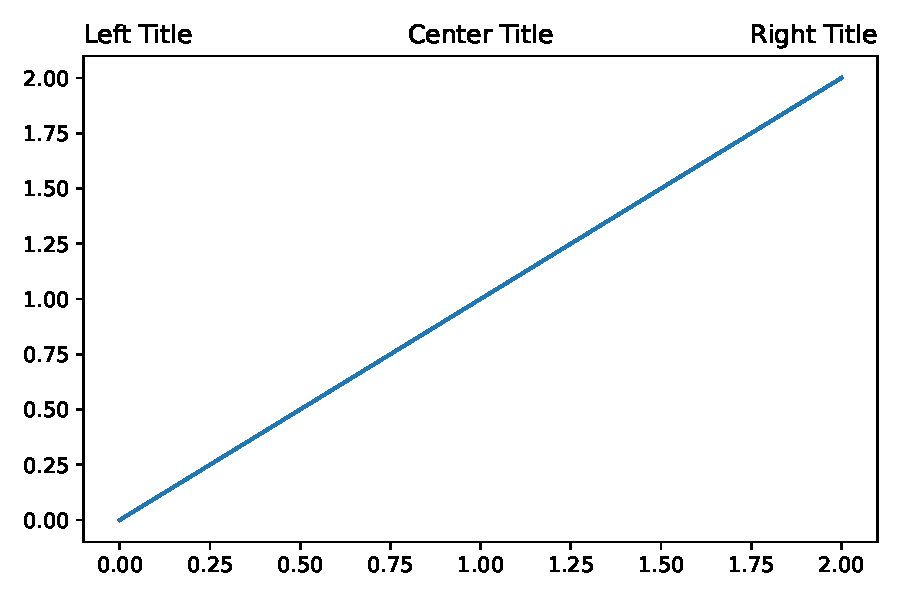
\includegraphics[width = .7\textwidth]{figures/proseplots/title-loc.pdf}
\end{center}


